% -----------------------------------------------------------------------------
% Introdução
% -----------------------------------------------------------------------------

\chapter{Introdução}
\label{chap:introducao}

\section{Motivação}
\label{sec:motivacao}

No contexto da análise de dados, diferentes ferramentas estão disponíveis para transformá-los em informação, contudo o uso dessas ferramentas na área da saúde ainda é pouco significativo \cite{galvao_desafios_2019}. Frente a uma tendência crescente de interconexão entre diferentes áreas do conhecimento e do potencial que a análise de dados possibilita para melhoria do sistema de saúde, se faz necessário propor e validar estratégias que permitam o avanço na integração de dados entre diferentes Sistemas de Informação em Saúde (SIS), e que facilitem o processamento e análise do grande volume de dados produzidos e disponibilizados nesses sistemas \cite{galvao_desafios_2019,mehta_concurrence_2018}.

Atualmente, conforme determinação do Decreto nº 8.777, de 11 de maio de 2016, que instituiu a Política de Dados Abertos do Poder Executivo Federal \cite{brasildisponibilidade2016}, diversos dados dos SIS são disponibilizados de forma pública. No entanto, apenas a disponibilização dos dados em si não garante que eles poderão ser analisados visando produzir informação relevante para as políticas públicas na área da saúde.

\section{Justificativa}
\label{sec:justificativa}


Alterações de governo e vertentes políticas mudam as prioridades de investimento e interesses o que faz com que o orçamento de alguns pilares de investimento e custo no país flutue como observado nos últimos 10 anos (Tabela \ref{tab:orcamento}). A disponibilidade de recursos financeiros efetivos para a ciência e tecnologia no Brasil têm oscilado. Nos anos de 2018 a 2021 sofreu reduções acentuadas, o que tornou ainda mais limitado o acesso a recursos que viabilizem a realização de análise dos dados em ferramentas e infra estruturas tradicionais ou ainda a proposta de novos.

Em uma avaliação simples desses dados, somado a variação do valor do dólar no mesmo periodo pode se observar (Figura \ref{fig:dolar}), pode ser ver um aumento de mais de $327\%$. Sendo que o orçamento não acompanhou essa flutuação. Essa ligação, apesar de não ser direta existe, sendo que em ciência e tecnologia equipamentos, licenças de \emph{software} etc utilizados no processamento de dados, são majoritariamente importadas, e portanto em dólar. Como o valor do orçamento efetivo por ano não acompanha o aumento do dólar, fica claro a perda de poder de compra, dado que a distribuição de verba do orçamento total tenha se mantido. 

Algo que valida a flutuação orçamentária é a queda consecutiva de orçamento desde 2018 (Figura \ref{fig:quedaorca}). Ainda podemos entender que mesmo em depois de 10 anos, temos um orçamento $2,32\%$ menor para ciência e tecnologia, o que impacta diretamente no financiamento de novos projetos, especialmente na compra de equipamentos que viabilizam pesquisas de larga escala ou que se valem de bases muito grandes como é o caso de bases como DataSUS e os diversos sistemas que compõem e, também, o banco de repasse orçamentário, limitando apenas para SUS, vindo de outras fontes como orçamento da união com pagamento diário e/ou semanal. Sem o poder computacional a disposição para estudo desses bancos, principalmente em instituições públicas, fica inviável a produção de conhecimento, a audição pela população e qualquer extração de informação viável. 

Essas limitações indiretas, impõem forte restrições no processo de avaliação e tomada de decisão embasada em dados. Ainda avaliando esse impacto econômico do problema descrito acima, é preciso pensar, como já discutido, a complexidade de tomada de decisões em saúde. Sem informações que embasem essa decisão fica restrita a capacidade de compreensão do senário nacional, sobre a situação de saúde pública. Quando leva-se em consideração que o SUS é um sistema subfinanciado, quando comparado a países que também possuem sistemas de saúde pública e gratuitas. O valor do orçamento por dia por pessoa é de apenas $R\$ 3,83$  o que é um preceito quando considera-se  restrição orçamentária do SUS por pessoa. Para entender a complexidade de um sistema tão abrangente é preciso avaliar sua escala. Mais de 152 milhões de pessoas utilizam exclusivamente o SUS como promotor de saúde. 

\begin{table}[htpb]
\centering
  \caption{Pagamento efetivo - Ministério da Ciência e Tecnologia}
  \label{tab:orcamento}
  \begin{tabular}{cc}
    \hline
    \textbf{Ano} & \textbf{Objetivo}    \\
    \hline
    2010         & R\$ 6.288.931.123,00 \\
    2011         & R\$ 5.918.584.706,00 \\
    2012         & R\$ 6.918.288.201,00 \\
    2013         & R\$ 7.787.464.592,00 \\
    2014         & R\$ 8.598.785.224,00 \\
    2015         & R\$ 7.964.319.815,00 \\
    2016         & R\$ 8.404.014.691,00 \\
    2017         & R\$ 9.085.620.227,00 \\
    2018         & R\$ 9.157.748.260,00 \\
    2019         & R\$ 8.812.096.752,00 \\
    2020         & R\$ 7.859.851.948,00 \\
    2021         & R\$ 6.142.873.884,00
  \end{tabular}
  \centering
  \begin{tablenotes}
  \centering
    \small
    \item{Fonte: SIOP consulta realizada em Janeiro de 2022}
  \end{tablenotes}
\end{table}

\begin{figure}[!h]
    \centering
    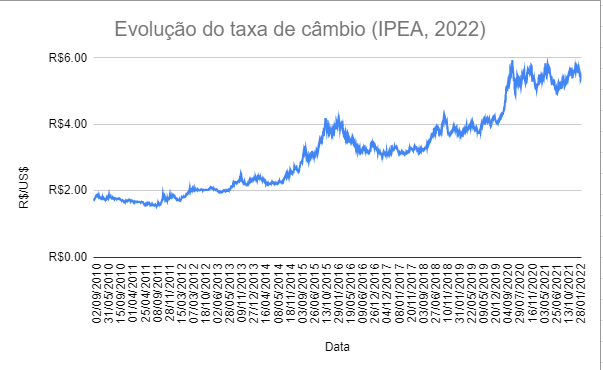
\includegraphics[width=0.8\textwidth]{04-figuras/dolar.png}
    \caption[Evolução do dólar/real na última década ]{Evolução do dólar/real na última década (Fonte: Feito pelo autor)}
    \label{fig:dolar}
\end{figure}
\begin{figure}[!h]
    \centering
    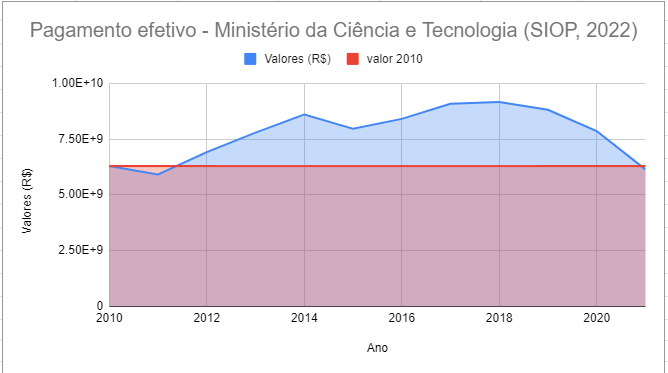
\includegraphics[width=0.8\textwidth]{04-figuras/compartive.png}
    \caption[Pagamento efetivo - Ministério da Ciência e Tecnologia ]{Pagamento efetivo - Ministério da Ciência e Tecnologia (Fonte: Feito pelo autor)}
    \label{fig:quedaorca1}
\end{figure}
\begin{figure}[!h]
    \centering
    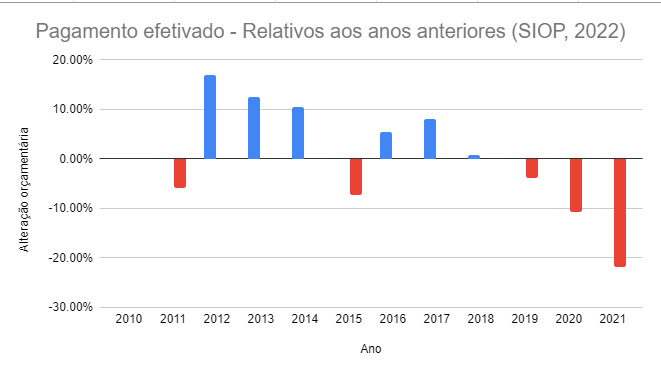
\includegraphics[width=0.8\textwidth]{04-figuras/compartive_last .png}
    \caption[Pagamento efetivo - Relativos aos anos anteriores ]{Pagamento efetivo - Relativos aos anos anteriores (Fonte: Feito pelo autor)}
    \label{fig:quedaorca}
\end{figure}

Tendo dado o contexto desse impacto na economia bem como na sociedade o presente trabalho se propõe a discutir alternativas e abordagens que amenizem impactos de orçamento disponibilizados pelo governo durante a viabilização de projetos de pesquisa que utilizam bases de dados tão grandes.

Nesse sentido, temos dois efeitos diretos:

\begin{itemize}
    \item Redução de fragilidade orçamentária
    \item Proposta de alternativas para análise de dados em saúde
\end{itemize}

A redução de fragilidade orçamentária se dá pela proposta de utilização de recursos já disponíveis e subutilizados, como \emph{desktops} de bibliotecas, laboratórios etc, por meio de ambientes virtualizados, compartilhando esses recursos com a orquestração das cargas de trabalhos de analise de dados. Para viabilizar essa proposta, o trabalho compara a performance de sistemas virtuais em computadores com baixo poder computacional, propondo assim uma forma de abordar, tanto o isolamento, para processos mais sensíveis, quanto a utilizam de recursos que já estão disponíveis o que garante o menor CAPEX possível para excussão do projeto de pesquisa. 

Para avaliação dessa alternativa toma-se como exemplo os bancos de “Vendas de Medicamentos Controlados e Antimicrobianos - Medicamentos Industrializados”, objeto deste trabalho, estão disponíveis cerca de 70 GB e com mais de 500 milhões de linhas de dados sobre a comercialização de medicamentos no país. Logo, tão importante quanto a disponibilidade pública dos dados, é fundamental encontrar estratégias técnicas e economicamente viáveis a fim de possibilitar que pesquisadores em todo o país possam contribuir com a análise e a interpretação desses dados, mesmo frente a baixa disponibilidade de recursos financeiros e de infraestrutura, como servidores de alta performance (HPC), por exemplo.

\section{Objetivos}
\label{sec:objetivos}
Diante disso, com a realização deste trabalho espera-se oferecer uma alternativa para análise de grandes volumes de dados que possua baixo custo financeiro, menor complexidade de configuração, maior efetividade (menor tempo de análise) e que não seja dependente da disponibilidade ou uso de recursos dedicados, como computadores de alta performance (HPC), às análises. A abordagem que irá se seguir é na utilização de alternativas \emph{open source} atualmente disponíveis que seja possíveis de serem utilizadas em computadores de baixo custo e menor poder computacional - ex.: \emph{OpenStack}, \emph{CloudStack} etc.

Deste modo, espera-se demonstrar comparativamente a implementação de uma solução para análise de dados em plataformas de orquestração de \emph{containers}, que permita recrutar computadores comuns para essa análise. E assim, espera-se, superar de maneira custo-efetiva um problema de restrição orçamentária e técnica para instituições públicas e grupos de pesquisa que realizam análises de grande volumes de dados. No caso deste trabalho, a aplicação está direcionada para a área da saúde, utilizando uma tecnologia já amplamente empregada no setor privado, o que viabiliza o suporte de estudantes e/ou profissionais das áreas de Engenharias e Computação. Espera-se, ainda, contribuir para que os dados públicos em saúde sejam analisados com  maior frequência e menor restrição, gerando indicadores melhores e atualizados para melhor tomada de decisão em saúde.

\section{Definição e abordagem}
\label{sec:abordagem}

A proposta do trabalho visa avaliar a utilização de \emph{cluster} de Kubernetes\textregistered \ como plataforma de orquestração de cargas de trabalho para processamento de dados em \emph{clusters }compostos por computadores de baixo custo ou reaproveitados.

Utilizando como carga de trabalho a análise de tendência de consumo de azitromicina no Brasil entre os anos de 2014 e 2021. Pretende-se utilizar, como principal resultado, a viabilidade de utilização de computadores do tipo \emph{desktop} para orquestração e análise de grades massas de dados como dados do SUS (Sistema Único de Saúde) garantindo assim viabilidade de trabalhos e proponto a utilização dessa plataforma em computadores menos específicos, como alternativa a HPC.

A utilização da plataforma visa validar seu uso para orquestração de tarefas em paralelo e precessamneto distribuído de dados, durante a análise, permitindo o uso simultâneo de diversas máquinas. Utilizando inicialmente 8 computadores com capacidades de processamento semelhantes a computadores desktop de 8-16 GB (Gigabytes) de RAM (Random Access Memory) e 4-8 vCPU (virtual Central Process Unit). Essa restrição  permitiram que uma analise de viabilidade para que o processmaneto e análise de grandes massas de dados (maiores que 50 GB) possam ser feitas sem o uso de HPC.

A abordagem de DevOps (BASS et al, 2015) para tornar o provisionamento, a integração e o \emph{deploy} da infra estrutura, bem como os componentes de análise desses utilizados neste trabalho incluem o conceito de CI (continuous integration), CD (continuous delivery).  IaC (Infrastructure as Code) visa tornar a configuração e disponibilização desse \emph{cluster} mais ágil, diminuindo assim a necessidade de operação e também de sua manutenção.

Para a análise de dados utilizando a estratégia descrita, propõe-se analisar as tendências de consumo da azitromicina no período de 2014 a 2021. Essa análise é objeto de carga de trabalho a ser orquestrado de maneira distribuída no \emph{cluster} para validação de seu desempenho nos ambientes propostos.

O trabalho não engloba a realização de interpretação da informação gerada pelo banco, garantindo, assim, apenas o resultado correto da análise citada como carga de trabalho para comparação. Também não está sendo proposta uma metodologia de análise do banco referenciado, mas a avaliação das tecnologias empregadas para orquestração das tarefas, comparação de desempenho entre as alternativas da implementação da plataforma e sua implementação como proposta para uso mais amplo nas instituições sob restrição orçamentária, com o fim de continuar a realizar análises de dados, ainda que sem hardware adequado.


\section{Organização do trabalho}
\label{sec:organizacaoTrabalho}

Este trabalho está dividido em 5 Capítulos. Esta Introdução apresentou o contexto geral do trabalho e tecnologias que serão avalias e citou possíveis problemáticas econômicas e sociais. 

O Capítulo 2 apresenta a fundamentação teórica e a revisão da literatura, discorrendo sobre as leituras que embasaram toda a construção do projeto, também aprofunda em conceitos necessários para as discussão e condução do trabalho. 

O Capítulo 3 apresenta a  metodologia utilizada para a construção dos componentes do projeto e a forma de avaliação de desempenho dos ambientes propostos bem como a forma de avaliação. 

O capitulo \ref{ch} apresenta os resultados obitidos tanto para orquestração das cargas de trabalho no ETL (extração, transformação e carga) e também os resultados obtidios apara a análise e processamento dos dados de consumo e prescrição obtidos para azitromicina no periodo descrito anteriormente.
discute os resultados adquiridos para a orequestração e analise dos dados de prescrição da azitromicia, além de suas interprestações. 

O capítulo \ref{chap:conclusao} apresenta as conclusões até a finalização do trabalho, discorre sobre as fases do TCC e também apresenta o que o aluno realizou ao longo da execução do trabalho, se a proposta do trabalho atingiu a espectativa como solução ao problema  proposto, além de possibilidades para trabalhos futuros. 